
\documentclass[conference]{IEEEtran}
\usepackage{cite}
\usepackage{graphicx}
\usepackage{amsmath}
\usepackage{enumerate}
\usepackage{xcolor}
\usepackage{pgfplots}
\usepackage{tikz}
\usepackage{listings}
\usepackage[linesnumbered]{algorithm2e}

\definecolor{bblue}{HTML}{4F81BD}
\definecolor{rred}{HTML}{C0504D}
\definecolor{ggreen}{HTML}{9BBB59}
\definecolor{ppurple}{HTML}{9F4C7C}

% correct bad hyphenation here
\hyphenation{op-tical net-works semi-conduc-tor}


\begin{document}

\title{PRECINCT:\@ An Incremental Approach for Preventing Clone Insertion at Commit Time}


\author{\IEEEauthorblockN{Mathieu Nayrolles, }
\IEEEauthorblockA{Software Behaviour Analysis (SBA) Research Lab\\
ECE, Concordia University\\
Montreal, Canada\\
m\_nayrol@ece.concordia.ca}
\and
\IEEEauthorblockN{Abdelwahab Hamou-Lhadj}
\IEEEauthorblockA{Software Behaviour Analysis (SBA) Research Lab\\
ECE, Concordia University\\
Montreal, Canada\\
abdelw@ece.concordia.ca}}

% make the title area
\maketitle

% As a general rule, do not put math, special symbols or citations
% in the abstract
\begin{abstract}
  Software clones are considered harmful since they may cause the same buggy code to appear in multiple places in the code, making software maintenance and evolution tasks challenging. Clone detection has been an active research field for almost two decades. Interestingly, most existing techniques focus on detecting clones after they are inserted in the code.  In this paper, we take another look at the clone detection problem by designing a novel approach for preventing the insertion of clones in the first place. Our approach, called PRECINCT (PREventing Clones INsertion at Commit Time),  detects efficiently  near-miss software clones at commit time by means of pre-commit hooks. This way, changes to the code are analysed and suspicious copies are flagged before they reach the central code repository in the version control system.  The application of PRECINCT to seven systems developed independently shows that PRECINCT achieves 100\% precision and a 93\% recall.



\end{abstract}


\IEEEpeerreviewmaketitle

\section{Introduction}
\label{sec:Introduction}


Code clones appear when developers reuse code with little to no modification to the original code.
Studies have shown  that clones can account for about 7\% to 50\% of code in a given software system\cite{Baker, StephaneDucasse}.
Developers often reuse code (and create clones) in their software on purpose\cite{Kim2005}.
Nevertheless, clones are considered a bad practice in software development since they can introduce new bugs in the code\cite{Kapser2006,Juergens2009,Li2006}. If a  bug is discovered in one segment of the code that has been copied and pasted several times, then the developers will have to remember the places where this segment has been reused in order to fix the bug in each of them.

In the last two decades, there have been many studies and tools that aim at detecting clones. They can be grouped into three categories. The first category includes techniques that treat the source code as text and use transformation and normalization  to compare various code fragments \cite{Johnson1994,Johnson1993, Cordy2011, Roy2008}. The second category includes methods that
use lexical analysis, where the source code is sliced into sequences of tokens, similar to the way a compiler operates\cite{Baker,Bakera,Baker2002,Kamiya2002,Li2006}. The tokens are used to compare code fragments. Finally, syntactic analysis has also been performed where the source code is converted into trees, more particularly abstract syntax tree (AST), and then the clone detection is performed using tree matching algorithms\cite{Baxter1998, Komondoor2000, Tairas2006, Falke2008}.

Despite the advances in clone detection, the use of exiting clone detection tools is not as widespread as one might think. The main factors that contribute to this are summarized in what follows \cite{Johnson2013}: These tools are known to output a large number of data, making it hard to understand and analyse their results. They tend to have a high amount of false positives.
They are also hard to configure and do not integrate well with the day-to-day workflow of a developer.

In this paper, we present PRECINCT (PREventing Clones INsertion at Commit Time) that focuses on preventing the insertion of clones in the first place at commit time, more particularly by  using pre-commit hooks capabilities of modern source code version control systems. A pre-commit hook is a process that one can implement to receive the latest modification to the source code done by a given developer just before the code reaches the central repository.  PRECINCT intercepts this modification and analyses its  content to see whether a suspicious clone has been introduced or not. A flag is raised if a code fragment is suspected to be a clone of an exiting code segment. In fact, PRECINCT itself is a pre-commit hook that detects clones that might have been inserted in the latest changes with regard to the rest of the source code. This said, only a fraction of the code is analysed and PRECINCT reduces the output by 70\%, compared to leading clone detection techniques such as \cite{Cordy2011}. Moreover, the detected clones are presented using a classical 'diff' output that developers are familiar with.  PRECINCTS is easy to use and configure. It only takes  one command line to configure PRECINCT. PRECINCT is also well integrated with the workflow of the developers since it leverages the pre-commit hook capability of modern source code version control systems such as Git and Jira.

We evaluated the effectiveness of PRECINCT using precision and recall on seven systems developed independently with a wide range of technologies. The results show that PRECINCT detects near-miss software clones before they reach the source version system with a 100\% precision and a 93\% recall while increasing the size of the repository by only 3\% to 5\%.

The rest of this paper is organized as follows: In Section~\ref{sec:Related Work}, we present the studies related to PRECINCT, with a particular emphasis on Nicad \cite{Cordy2011}, used to build PRECINCT. Then, in Section~\ref{sec:The PRECINCT Approach}, we present the PRECINCT approach. The evaluation of PRECINCT is the subject of  Section~\ref{sec:Experimentations}.
Finally, we propose concluding remarks in Section~\ref{sec:Conclusion}.

\section{Related Works}
\label{sec:Related Works}

\cite{Lague}


\section{The PRECINCT Approach}
\label{sec:The PRECINCT Approach}

\begin{figure*}
  \centering
    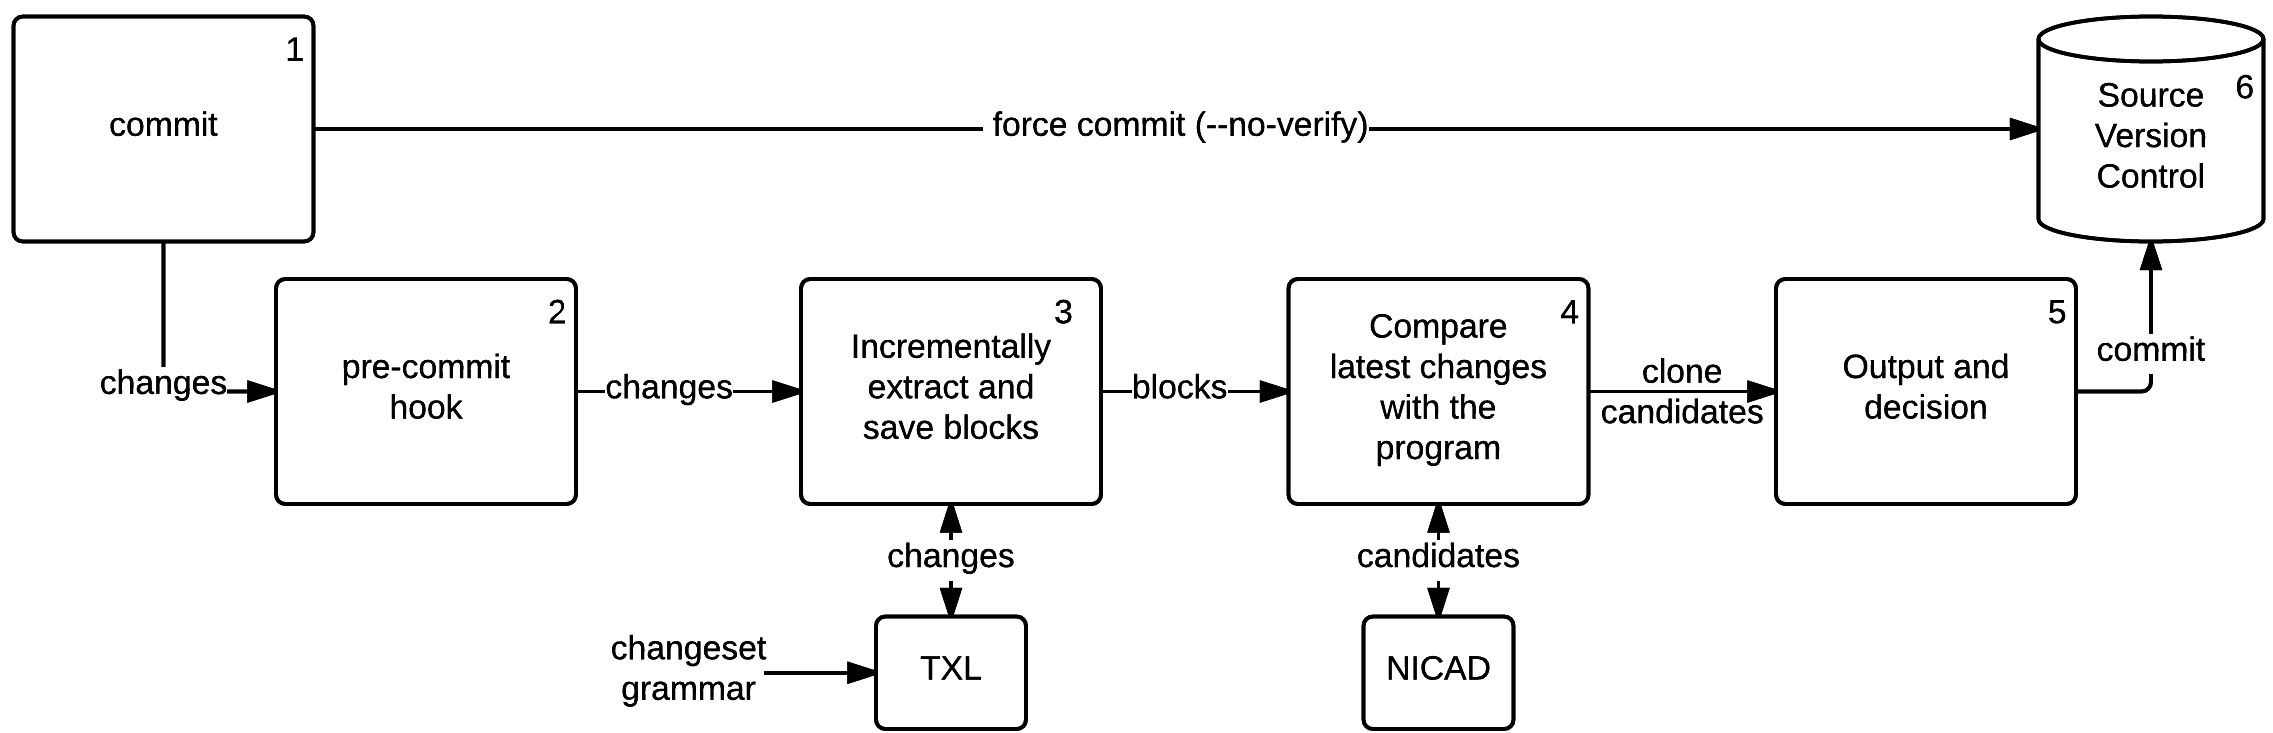
\includegraphics[width=\textwidth]{media/approach.png}
    \caption{ Overview of the PRECINCT Approach.\label{fig:precinct-approach}}
\end{figure*}

The PRECINCT approach is composed of six steps. The first step is the commit step where developers send their latest change to the central repository and the last step is the reception of the commit by the central repository. The second step is the pre-commit hook which kicks in as the first operation when one wants to commit. The pre-commit hook has access to the changes in terms of files that have been modified, more specifically, the lines that have been modified. The modified lines of the files are sent to TXL\cite{Cordy2006a} for block extraction. Then, the blocks are compared to previously extracted blocks in order to identify candidate clones  using Nicad\cite{Cordy2011}. Finally, the output of Nicad is further refined and presented to the user for a decision round. These steps are discussed in more detail in the following subsections.

\subsection{Commit}
\label{sub:Commit}

In version control systems, a commit adds the latest changes made to the source code to the repository, making these changes part of the head revision of the repository. Commits in version control systems are kept in the repository indefinitely. Thus, when other users do an update or a checkout from the repository, they will receive the latest committed version, unless they wish to retrieve a previous version of the source code in the repository. Version control systems allow rolling back to previous versions easily. In this context, a commit within a version control system is protected as it is easily rolled back, even after the commit has been done.

\subsection{Pre-Commit Hook}
\label{sub:Pre-Commit Hook}

Hooks are custom scripts set to fire off when certain important actions occur.
There are two groups of  hooks: client-side and server-side. Client-side hooks are triggered by operations such as committing and merging, whereas server-side hooks run on network operations such as receiving pushed commits. These hooks can be used for all sorts of reasons (GIVE ONE OR TWO EXAMPLES).


The pre-commit hook is run first, before one even types in a commit message. It is used to inspect the snapshot that is about to be committed. This is used to allow developers to check if they have not forgotten anything, to run tests, or to examine whatever the need to inspect the code. Exiting [WAHAB: I DO NOT UNDERSTAND THIS SENTENCE] non-zero from this hook aborts the commit, although one can bypass it with a no-verify commit (a feature that exists in Git and other version systems).
Developers can do things like check for code style (run lint or something equivalent), check for trailing white spaces (the default hook does exactly this), or check for appropriate documentation on new methods.

PRECINCT is a set of bash scripts where the entry point of these scripts lies in the pre-commit hooks. Pre-commit hooks are easy to create and implement as depicted in Listing~\ref{gitprehook}. The pre-hook is shipped in version control systems like Git\footnote{https://git-scm.com/}. Note that even though we use Git as the main version control to present PRECINCT, we believe that the techniques presented in this paper are readily applicable to other version control systems. From lines 3 to 11, the script identifies if the commit is the first one in order to select the revision to work against. Then, in Lines 18 and 19, the script checks for trailing whitespace and fails if any are found.

\noindent\begin{minipage}{0.90\linewidth}

  \lstinputlisting[language=Bash, firstnumber=1, numbers=right, stepnumber=1,leftmargin=30, label=gitprehook, caption=Git Pre-Commit Hook Sample]{media/pre-commit.sample}

\end{minipage}

For PRECINCT to work, we just have to add the call to our script suite instead or in addition of the whitespace check.

\subsection{Extract and Save Blocks}
\label{sub:Extract and Save Blocks}

A block is a set of consecutive lines of code that will be compared to all other blocks in order to identify clones.
To achieve this critical part of PRECINCT, we rely on TXL\cite{Cordy2006a}, which is a first-order functional programming over linear term rewriting, developed by Cordy et al.\cite{Cordy2006a}. For TXL to work, one has to write a grammar describing the syntax of the source  language and the transformations needed. TXL has three main phases: \textit{parse, transform}, \textit{unparse}. In the parse phase, the grammar controls not only the input but also the output form. Listing~\ref{txlsample} --- extracted from the official documentation\footnote{http://txl.ca} --- shows a grammar matching a \textit{if-then-else} statement in C with some special keywords: [IN] (indent), [EX] (exdent) and [NL] (newline) that will be used for the output form.

\noindent\begin{minipage}{0.90\linewidth}

  \lstinputlisting[language=Bash, firstnumber=1, numbers=right, stepnumber=1,leftmargin=30, label=txlsample, caption=Txl Sample Sample]{media/txl.sample}

\end{minipage}

Then, the \textit{transform} phase will, as the name suggests, apply transformation rules that can, for example, normalize or abstract the source code. Finally, the third phase of TXL,  called \textit{unparse}, unparses the transformed parsed input in order to output it. Also, TXL supports what the creators call Agile Parsing\cite{Dean}, which allow developers to redefine rules of the grammar and, therefore, apply different rules than the original ones.


PRECINCT takes advantage of that by redefining the blocks that should be extracted for the purpose of clone comparison, leaving out the  blocks that are out of scope.  More precisely, before each commit, we only extract the blocks belonging to the modified parts of the source code, hence reducing the size of the output, a common issue of clone detection techniques as discussed in the introductory section. 

We have selected TXL for several reasons. First, TXL is easy to install and to integrate with a developer workflow. Second, it was relatively easy to create a grammar that accepts commits as input. This is because TXL is shipped with C, Java, Csharp, Python and WSDL grammars that define all the particularities of these languages, with the ability to customize these grammar to to accept changesets (chunks of the modified source code that includes the added, modified, and deleted lines) instead of the whole code.


Algorithm~\ref{alg:extract} presents an overview of the "extract" and "save" blocks operations.

\begin{algorithm}[H]
 \KwData{$Changeset[]$ changesets\;
 $Block[]$ prior\_blocks\;
 $Boolean$ compare\_history\;
 }
 \KwResult{Up to date blocks of the systems}
 \For{$i \leftarrow 0$ \KwTo$size\_of~changesets$}{
    Block[] blocks $\leftarrow$ $extract\_blocks(changesets)$\;
    \For{$j \leftarrow 0$ \KwTo$size\_of~blocks$}{
       \If{not $compare\_history$ AND $blocks[j]$ overrides one of $prior\_blocks$}{
          delete $prior\_block$\;
       }
       write $blocks[j]$\;
    }
 }

 \SetKwProg{myproc}{Function}{ $~extract\_blocks(Changeset~cs)$}{}
   \myproc{\proc{}}{

   \uIf{$cs~is~unbalanced~right$}{$cs \leftarrow expand\_left(cs)$\;}

   \ElseIf{$cs~is~unbalanced~left$}{$cs \leftarrow expand\_right(cs)$\;}

   \nl\KwRet$txl\_extract\_blocks(cs)$\;
   }

 \caption{Overview of the Extract Blocks Operation\label{alg:extract}}
\end{algorithm}

This algorithm receives as arguments, the changesets, the blocks that have been previously extracted and a boolean named compare\_history.
Then, from Lines 1 to 9 lie the $for$ loop that iterates over the changesets. For each changeset (Line 2), we extract the blocks by calling the $~extract\_blocks(Changeset~cs)$ function.
In this function, we expand our changeset to the left and to the right in order to have a complete block.
As depicted by Listing~\ref{commitsample}, changesets contain only the modified chunk of code and not necessarily complete blocks. Indeed, we have a block from Line 3 to Line 6 and deleted lines from Line 8 to 14.
However, in Line 7 we can see the end of a block but we do not have its beginning. Therefore, we need to expand the changeset to the left in order to have syntactically correct blocks.
We do so by checking block's beginning and ending, \{ and \} in C for example.
Then, we send these expanded changesets to TXL for block extraction and formalization.

\noindent\begin{minipage}{0.90\linewidth}

  \lstinputlisting[language=Bash, firstnumber=1, numbers=right, stepnumber=1,leftmargin=30, label=commitsample, caption=Changeset c4016c of monit]{media/commit.sample}

\end{minipage}


For each extracted block, we check if the current block overrides (replaces) a previous block (Line 4).
In such a case, we delete the previous block as it does not represent the current version of the program anymore (Line 5).
Also, we have an optional step in PRECINCT defined in Line 4. The compare\_history is a condition to delete overridden blocks.

[WAHAB: I DON'T UNDERSTAND THE FOLLOWING 3 SENTENCES. PLEASE REPHRASE]
We believe that overridden blocks have been so far a good reason (bug, default, removed features, \ldots) and if a newly inserted block matches an old one, it could be worth knowing to improve the quality of the system at hand.
This feature is deactivated by default.

In summary, this step receives the files and lines, modified by the latest changes made by the developer and produces an up to date block representation of the system at hand. The blocks can be analysed in the next step to discover potential clones.

\subsection{Compare Extracted Blocks}
\label{sub:Compare Extracted Blocks}

In order to compare the extracted blocks and detect potential clones we could only rely on text-based techniques.
Indeed, lexical and syntactic techniques would be of no help as they require a complete program to work, a program that compiles.
In the relatively wide-range of tool and technics that exist to detect clone by considering code as text \cite{Johnson1993,Johnson1994,Marcus,Manber1994,StephaneDucasse,Wettel2005}, we choose NICAD \cite{Cordy2011} for several reasons.
First NICAD is built on top of TXL and as we also use TXL on the previous step, the integration between the step was made easy.
Second, NICAD, is able to detect all types of clones.

NICAD (Accurate Detection of Near-miss Intentional Clones) works in three phases: \textit{Extraction}, \textit{Comparison} and \textit{Reporting}.
During the \textit{Extraction} phase in all potential clones are identified, pretty-printed and extracted.
We do not use the \textit{Extraction} phase of NICAD as it has been built to work on programs that are syntactically correct and changesets are not.
We replaced NICAD's \textit{Extraction} phase by our own processes described in the previous section.

In the \textit{Comparison} phase, extracted blocks are transformed, clustered and compared in order to find potential clones.
Using TXL sub-programs, blocks go through a process called pretty-printing where they are stripped of formatting and comments.
Indeed, when code cloned, some comments, indentation or spacing are changed according to the new context this code will be used in.
This pretty-printing process ensures that all code will have the same spacing and formatting and ease the comparison.
Furthermore, in the pretty-printing process, statements can be broken down into several lines.
Table~\ref{tab:pretty-printing} shows how this can improve the accuracy of clone detection with three \texttt{for} statements, \texttt{ for (i=0; i<10; i++)}, \texttt{for (i=1; i<10; i++)} and \texttt{ for (j=2; j<100; j++)}.
The pretty-printing allows NICAD to detect segment 1 and 2 as a clone pair because only the initialization of $i$ changed.
This specific example would not have been marked as a clone by other line based tools we tested such as Duploc\cite{Ducasse1999}.
In addition to the pretty-printing, code can be normalized and filtered to detect different classes of clones and match user preferences.

\begin{table}[]
\centering
\caption{Pretty-Printing Example\cite{Iss2009}}
\label{tab:pretty-printing}
\resizebox{0.5\textwidth}{!}{%
\begin{tabular}{l|l|l|l|l|l}
Segment 1          & Segment 2          & Segment 3           & S1 \& S2 & S1 \& S3 & S2 \& S3 \\ \hline \hline
for (              & for (              & for (               & 1        & 1        & 1        \\
i = 0;             & i = 1;             & j = 2;              & 0        & 0        & 0        \\
i \textgreater 10; & i \textgreater 10; & j \textgreater 100; & 1        & 0        & 0        \\ 
i++)               & i++)               & j++)                & 1        & 0        & 0        \\ \hline \hline
\multicolumn{3}{c|}{Total Matches}                            & 3        & 1        & 1        \\ \hline
\multicolumn{3}{c|}{Total Mismatches}                         & 1        & 3        & 3
\end{tabular}
}
\end{table}


Finally, the extracted, pretty-printed, normalized and filtered blocks are marked as potential clones using a Longest Common Subsequence (LCS) algorithm\cite{Hunt1977}.
Then, a percentage of unique statement can be computed and, depending a given threshold (see Section \ref{sec:Experimentations}), the blocks are marked as clones.

The last step of NICAD, which acts as our clone comparison engine, is the \textit{reporting}.
However, we wanted PRECINCT to address the \textit{massive output} concern and  implemented our own reporting system which also falls into the \textit{workflow} of developers.
This reporting system is the subject of the next section.

As a summary, this step receives potentially expanded and balanced blocks from the extraction step.
Then, the blocks are pretty-printed, normalized, filtered and fed to an LCS algorithm in order to detect potential clones.

\subsection{Output and Decision}
\label{sub:Output and Decision}

In this final step, we report the result of the clone detection with regards to the latest changes of the developer.
The process here is very simple.
Every change made by the developers has been through the previous steps and might have been marked as clones to another part of the system at hand.
For each file that is suspected to contain a clone, one line is printed to the command line with the following options: (I) Inspect, (D) Disregard, (R) Remove from the commit as shown by Figure X.

(I) Inspect will cause a diff-like visualization of the suspected clones (Figure Y) while (D) disregard will simply ignore the finding.
To integrate PRECINCT in the workflow of developer will also propose the (R) remove option.
This option will simply remove the suspected file from the commit that is about to be sent to the central repository.
Also, if the user types an option key twice, e.g. II, DD or RR, then, the option will be applied to files.
For instance, if the developer type DD at any one point, all the findings will be disregarded and the commit will be allowed to go through.







\section{Experimentations}
\label{sec:Experimentations}

\section{Conclusion}
\label{sec:Conclusion}







\bibliographystyle{IEEEtran}
\bibliography{library.bib}


\end{document}
